\documentclass{beamer}
\usepackage[utf8]{inputenc}
\usepackage{palatino}
\usepackage{subfig}
\usepackage{amsmath}
\usepackage{amssymb}
\usepackage{dsfont}
\usepackage{multimedia}
\usepackage{hyperref}

\usetheme{Copenhagen}
\usecolortheme{crane}

% www.sharelatex.com/learn/Beamer

\title{Computing Entropies with Nested Sampling}
\author{Brendon J. Brewer}
\institute{Department of Statistics\\
The University of Auckland}
\date{\color{blue}\bf \url{https://www.stat.auckland.ac.nz/~brewer/}}

\begin{document}

\frame{\titlepage}


% New slide
\begin{frame}
\frametitle{The fundamental theorem of information theory}

\end{frame}


% New slide
\begin{frame}
\frametitle{The fundamental theorem of information theory}

\begin{block}{Theorem}
If you take the log of a probability, it seems like you understand profound
truths.
\end{block}


\end{frame}


% New slide
\begin{frame}
\frametitle{Shannon entropy}

Consider a discrete probability distribution with probabilities
$\boldsymbol{p} = \{p_i\}$. The Shannon entropy is
\begin{align}
H(\boldsymbol{p}) &= -\sum_i p_i \log p_i
\end{align}

It is a real-valued property of the distribution.
There is also relative entropy / KL divergence,
which is a function of two distributions, and is more fundamental.

\end{frame}



% New slide
\begin{frame}
\frametitle{Entropy quantifies uncertainty}
If there are just $N$ equally likely possibilities,
i.e., $p_i = 1/N$, then $H = \log N$. \vspace{0.5em}

\begin{center}
\includegraphics[width=0.6\textwidth]{entropy3.pdf}
\end{center}

\end{frame}


% New slide
\begin{frame}
\frametitle{What about densities?}
We get `differential entropy'

\begin{align}
H = - \int_{\textnormal{all }x} f(x) \log f(x) \, dx
\end{align}

This generalises log-volume, as defined {\bf with respect to} $dx$.
\pause
\begin{alertblock}{Important}
Differential entropy is {\em coordinate-system dependent}.
\end{alertblock}

\end{frame}






% New slide
\begin{frame}
\frametitle{Some entropies in Bayesian statistics}
Written in terms of parameters $\theta$ and data
$d$, for Bayesian purposes. These are relevant to
experimental design...

\begin{enumerate}
\item<2-> Entropy of the prior for the parameters $H(\theta)$
\item<3-> Entropy of the conditional prior for the data $H(d | \theta)$
\item<4-> Entropy of the posterior $H(\theta | d)$
\item<5-> Entropy of the prior for the data $H(d)$
\end{enumerate}

\pause
\pause
\pause
\pause
\pause

\begin{block}{Remark}
{\em Conditional entropies} such as (2) and (3)
are defined using an expectation over the second argument
(the thing conditioned on).
\end{block}

\end{frame}


% New slide
\begin{frame}
\frametitle{Hard integrals}

E.g.
\begin{align}
H(\theta|d) &= -\int p(d) \int p(\theta|d) \log p(\theta|d) \, d\theta \, dd \\
            &= -\int p(d) \int p(\theta|d)
                    \log\left[\frac{p(\theta)p(d|\theta)}{p(d)}\right] \, d\theta \, dd
\end{align}

But $p(d)$, sitting there inside a logarithm, is already supposed to be
a hard integral (the marginal likelihood / evidence)...

\begin{align}
p(d) &= \int p(\theta) p(d|\theta) \, d\theta
\end{align}

It's even worse with nuisance parameters.

\end{frame}



% New slide
\begin{frame}
\frametitle{Marginal Likelihood Integral}
Nested Sampling was invented in order to do this hard integral
\begin{align}
p(d) &= \int p(\theta) p(d|\theta) \, d\theta
\end{align}

or
\begin{align}
Z &= \int \pi(\theta) L(\theta) \, d\theta
\end{align}
where $\pi=$ prior, $L=$ likelihood.
This is hard because $\pi \implies$ a heavy-tailed
distribution of $L$-values.

\end{frame}


% New slide
\begin{frame}
\frametitle{Nested Sampling}
Nested Sampling takes the original problem and constructs
a 1D problem from it.

\begin{align}
Z = \int_0^1 L(X) dX
\end{align}
where
\begin{align}
X(\ell) &= \int_{L(\theta) > \ell} \pi(\theta) \, d\theta
\end{align}

\begin{block}{The meaning of $X$}
$X(\ell)$ is the amount of prior mass whose likelihood exceeds
$\ell$. As $\ell$ increases, $X$ decreases.
\end{block}

\end{frame}


\begin{frame}
\frametitle{Nested Sampling}

\begin{center}
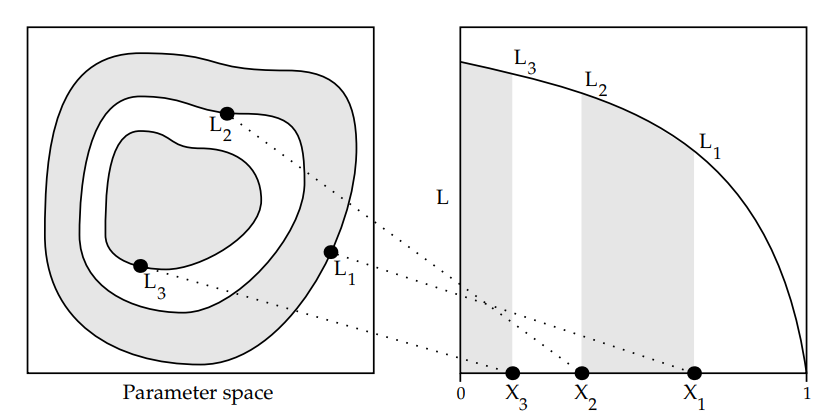
\includegraphics[width=0.8\textwidth]{skilling.png}

Figure from Skilling (2006).
\end{center}

Since $X(\ell)$ is the CDF of $L$-values implied by $\pi$,
points $\theta \sim \pi$ have a uniform distribution over $X$.

\end{frame}


% New slide
\begin{frame}
\frametitle{The sequence of $X$-values}
The sequence of $X$ values, if you transform them, have
a Poisson process distribution with rate $N$.

\begin{align}
-\ln(X_1) &\sim \textnormal{Exponential}(N) \\
-\ln(X_2) &\sim -\ln(X_1) + \textnormal{Exponential}(N) \\
-\ln(X_3) &\sim -\ln(X_2) + \textnormal{Exponential}(N) 
\end{align}

(forgive the notational abuse)
\pause
\begin{block}{Remark}
Number of iterations taken to exceed a certain likelihood
$\ell$, divided by number of particles $N$,
is an unbiased estimator of $-\ln X(\ell)$.
\end{block}


\end{frame}

%% New slide
%\begin{frame}
%\frametitle{Poisson process view of NS}

%The number of NS iterations taken
%to enter a small region (defined by a likelihood threshold) 
%is an unbiased estimator of the log-probability
%of that region!\vspace{0.7em}

%Also, $\pi(\theta)$ can be any distribution (needn't be
%a prior) and $L(\theta)$ any scalar function. Opportunities here...

%\end{frame}


% New slide
\begin{frame}
\frametitle{My algorithm}
To compute $H(\theta) = -\int f(\theta) \log f(\theta) \, d\theta$
when $f$ can be sampled but not evaluated:

\begin{enumerate}
  \item<2-> Generate a `reference point' $\theta_{\rm ref}$ from $f$
  \item<3-> Do a Nested Sampling run with $f$ as ``prior'' and
            minus the distance to $\theta_{\rm ref}$ as
            ``likelihood''.
  \item<4-> Measure how many NS iterations were needed to make the
            distance to $\theta_{\rm ref}$ really small, and divide
            by $N$. That gives an
            unbiased estimate of the
            log-prob near $\theta_{\rm ref}$.
  \item<5-> Repeat steps 1--3 many times.
  \item<6-> Average the estimated log-probs, then apply corrections
            to convert to density.
\end{enumerate}
\end{frame}


% New slide
\begin{frame}
\frametitle{My algorithm}

\begin{center}
\includegraphics[width=0.7\textwidth]{movie/image000001.png}
\end{center}

\end{frame}



% New slide
\begin{frame}
\frametitle{My algorithm}

\begin{center}
\includegraphics[width=0.7\textwidth]{movie/image000021.png}
\end{center}

\end{frame}



% New slide
\begin{frame}
\frametitle{My algorithm}

\begin{center}
\includegraphics[width=0.7\textwidth]{movie/image000041.png}
\end{center}

\end{frame}


% New slide
\begin{frame}
\frametitle{My algorithm}

\begin{center}
\includegraphics[width=0.7\textwidth]{movie/image000061.png}
\end{center}

\end{frame}



% New slide
\begin{frame}
\frametitle{Movie}

Play movie.mkv

(It's also on YouTube)

\end{frame}


% New slide
\begin{frame}
\frametitle{Toy experimental design example}
Two observing strategies --- even and uneven.
Which is better for measuring a period?

\begin{center}
\includegraphics[width=0.8\textwidth]{../paper/figures/sinewave.pdf}
\end{center}

\end{frame}


% New slide
\begin{frame}
\frametitle{Specifics}
Let $\tau = \log_{10}(\textnormal{period})$.\vspace{0.5em}

I knew $H(\tau)$ because I chose
the prior. I used the algorithm to estimate $H(\tau | d)$,
so marginal posteriors
were the distributions whose entropies I estimated\footnote{If you only
care about one parameter, define your distance function in terms of that
parameter only!}.\vspace{0.5em}

I then computed the mutual information
\vspace{0.5em}

\begin{align}
I(\tau; d) &= H(\tau) - H(\tau | d)
\end{align}

\end{frame}

% New slide
\begin{frame}
\frametitle{Result}

\begin{align}
I_{\rm even}   &= 5.441 \pm 0.038 \textnormal{ nats}\\
I_{\rm uneven} &= 5.398 \pm 0.038 \textnormal{ nats}
\end{align}

i.e., any difference is trivial.

\end{frame}


% New slide
\begin{frame}
\frametitle{Paper/software/endorsement}

{\color{blue}\bf \url{http://www.mdpi.com/1099-4300/19/8/422}
\url{https://github.com/eggplantbren/InfoNest}}
\vspace{0.5cm}

\begin{center}
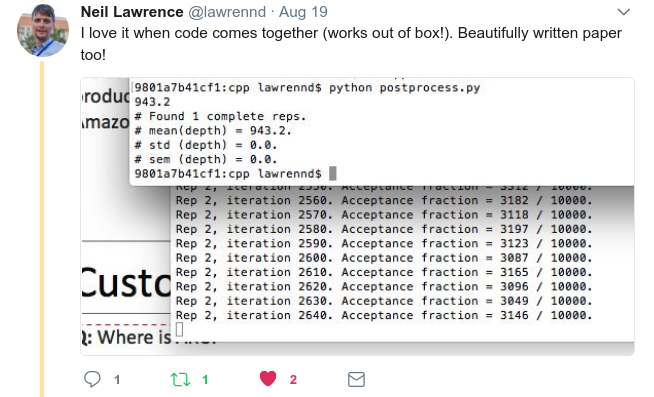
\includegraphics[width=0.7\textwidth]{lawrence.png}
\end{center}

\end{frame}



% New slide
\begin{frame}
\frametitle{Thanks}


Ruth Angus (Flatiron Institute),
Ewan Cameron (Oxford), James Curran (Auckland), Tom Elliott (Auckland),
David Hogg (NYU), Kevin Knuth (SUNY Albany),
Thomas Lumley (Auckland),
Iain Murray (Edinburgh), John Skilling
(Maximum Entropy Data Consultants), Jared Tobin ({\tt jtobin.io}).


\end{frame}




%% New slide
%\begin{frame}
%\frametitle{References I.}

%On the connection between Shannon entropy and thermodynamic entropy,
%see: \vspace{2em}

%{\tiny Jaynes, Edwin T. ``Gibbs vs Boltzmann entropies.''
%American Journal of Physics 33, no. 5 (1965): 391-398. \\

%Brewer, Brendon J. ``Unscrambling the Second Law of Thermodynamics''
%{\color{blue}
%  \url{https://quillette.com/2016/01/28/unscrambling-the-second-law-of-thermodynamics}
%}
%} % tiny

%\end{frame}

%% New slide
%\begin{frame}
%\frametitle{Statements and questions}
%Consider a problem with three mutually exclusive, exhaustive possibilities
%\texttt{a}, \texttt{b}, and \texttt{c}.


%\begin{center}
%  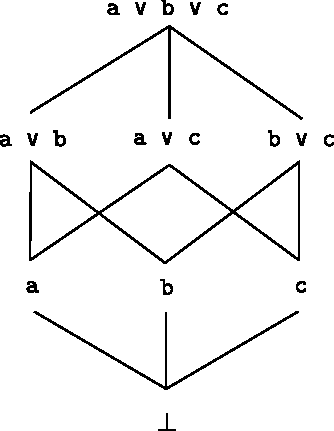
\includegraphics[width=0.3\textwidth]{lattice1.pdf}
%\end{center}

%\end{frame}



\end{document}


